\documentclass[tikz,10pt,a4paper]{article}
\usepackage{fullpage}
\usepackage[utf8]{inputenc}
\usepackage[T2A]{fontenc}
\usepackage{graphics,graphicx,epsfig}
\usepackage{amssymb,amsfonts,amsthm,amsmath,mathtext,cite,enumerate,float}
\usepackage[english,russian]{babel}
\usepackage[all]{xy}
\usepackage{morefloats}
\usepackage{pgf}
\usepackage[debug,outputdir={docgraphs/}]{dot2texi}
\usepackage{tikz}
\usepackage{scalefnt}
\usepackage{listings}
\usepackage{float}
\usepackage{verbatim}
\usepackage{placeins}
\usepackage{url}
\usepackage{babelbib}
\usepackage{pbox}
\usepackage{grffile}
\usepackage{color}
\usepackage{xfrac}
\usepackage{comment}
\usepackage{rotating}
\usepackage{slashbox}
\usepackage{caption}
\usepackage{subcaption}
\usetikzlibrary{arrows,shapes,intersections,decorations.markings,calc}

\makeatletter
\def\@settitle{\begin{center}%
    \baselineskip14\p@\relax
    \bfseries
    \@title
  \end{center}%
}

\makeatother

\newcommand{\bomega}{\boldsymbol{\omega}}

\begin{document}

\begin{center}
  \MakeUppercase{Модификация функционала качества в задачах нелинейной регрессии для учета гетероскедастичных погрешностей измеряемых данных}

  \bigskip
  Г.\,И.~Рудой\footnote{Московский физико-технический институт, 0xd34df00d@gmail.com}
\end{center}

\begin{abstract}
  Рассматривается задача восстановления нелинейной
  регрессионной зависимости по данным, имеющим погрешности определения как зависимых,
  так и независимых переменных, при этом распределения погрешностей
  различных измерений могут иметь различную дисперсию.
  Предлагается модифицированный функционал среднеквадратичной ошибки,
  учитывающий погрешности определения независимых переменных и различные распределения
  погрешностей в разных точках.
  Приводятся результаты численного моделирования на данных, полученных в ходе
  эксперимента по измерению зависимости мощности лазера от прозрачности
  резонатора.
  Рассматривается сходимость вектора параметров, минимизирующего
  предлагаемый функционал качества, к оптимальному для классического
  функционала среднеквадратичной ошибки.
  Сравнивается сходимость параметров, оптимальных для предлагаемого
  и классического функционалов, к некоторым <<истинным>> параметрам
  модели на данных, сгенерированных согласно этим <<истинным>> параметрам и зашумленным
  согласно предположениям о погрешностях измерений, в зависимости от параметров этих
  погрешностей.

  \textbf{Ключевые слова}: \emph{гетероскедастичные ошибки,
  ошибки измерения независимых переменных, символьная регрессия, нелинейная регрессия.}
\end{abstract}

\section{Введение}

В ряде приложений (например, \cite{Gladun2004Labs,Rudoy15MonteCarlo})
возникает задача нахождения оптимальных
коэффициентов $\bomega$ некоторой регрессионной модели $f$, заданной
в виде аналитической формулы, по набору экспериментальных данных. Для этого
в предположении о нормальном распределении регрессионных остатков
строится функционал $\sum_i (y_i - f(x_i, \bomega))^2$,
представляющий сумму квадратов отклонений экспериментальных точек $y_i$ от
значения регрессионной кривой $f(x, \bomega)$ в точке $x_i$,
и находится вектор параметров $\bomega$, его минимизирующий.

Однако, данный функционал корректен только для точно измеренных независимых
переменных и гомоскедастичных ошибок измерения зависимой переменной:
в частности, для линейных моделей соответствующая оценка параметров является
несмещенной, состоятельной и наиболее эффективной только при выполнении этих
условий. В случае нелинейных моделей вывод функционала среднеквадратичной
ошибки согласно методу наибольшего правдоподобия также опирается на
эти предположения (с обобщением в виде взвешенного метода наименьших
квадратов в случае различных стандартных отклонений зависимой
переменной).
Иными словами, предполагается существование лишь ошибок измерения зависимой
переменной, распределение которых принимается одинаковым.

На практике, как правило, это предположение не выполняется,
особенно при измерении некоторой зависимости в достаточно широких диапазонах.
Например, в задаче нахождения зависимости коэффициента преломления $n$ прозрачного
полимера от длины волны $\lambda$ погрешности измерения каждого физического
параметра в различных точках, вообще говоря, различны\cite{Rudoy15MonteCarlo}.
Так, если для измерения длины волны $\lambda$ используется дифракционная
решетка, то постоянной является относительная погрешность определения длины волны
$\frac{\sigma_{\lambda_i}}{\lambda_i} \approx \text{const}$, и, следовательно,
погрешность определения длины волны зависит от самой длины волны. Подобная ситуация
фиксированной относительной (а не абсолютной) ошибки является типичной для
физических экспериментов.

Таким образом, возникает задача поиска оптимальных коэффициентов регрессионной
формулы с учетом различающихся погрешностей измерения в различных экспериментальных точках.
Для некоторых частных случаев эта задача уже решена.

Так, всеобъемлющий обзор методов решения этой задачи
в случае линейной регрессии приведен в работе \cite{gillard2006historical}.
В частности, для линейных моделей рассматривается более общая задача,
когда распределение ошибок не является точно известным.
Однако, по крайней мере, для ряда методов априорная информация все
равно необходима, как то значение отношения стандартных отклонений
зависимой и независимой переменных
в случае регрессии Деминга \cite{Deming1943Statistical}
либо наличие инструментальных переменных
при использовании одноименного метода \cite{Bowden1990Instrumental}.
Отметим, что дополнительная априорная информация необходима
для обеспечения возможности однозначного определения параметров
модели, иначе модель становится неидентифицируемой. При этом
условие идентифицируемости модели для случая многомерной
линейной регрессии в общем виде до сих пор неизвестно
\cite{Bekker1986Comment}.

Обзор методов решения аналогичной задачи для случая нелинейной
регрессии приведен в книге \cite{Carrol06MeasurementErrors}.
Так, например, метод инструментальных переменных
обобщается на случай нелинейных моделей, при этом,
опять же, требуется наличие дополнительных наблюдаемых переменных,
пропорциональных регрессору с точностью до некоторой аддитивной
ошибки.
Заметим, что условия идентифицируемости модели при этом неизвестны.

Кроме того, в ряде работ изучаются конкретные нелинейные
регрессионные модели, и соответствующие ошибки измерений
предполагаются экспертно заданными.

Например, в \cite{jukic2013nonlinear} рассматривается модель Басса,
описывающая динамику процесса распространения новых потребительских продуктов,
для которой вводится предположение о неравной точности измерений в различных
экспериментальных точках, что описывается различными весовыми коэффициентами при
соответствующих регрессионных остатках. При этом весовые коэффициенты имеют достаточно
общий вид и вводятся произвольно в виде экспертно указанных значений.

Другим примером является \cite{jukic2010nonlinear}, где рассматривается задача оценки коэффициентов
трехпараметрического распределения Вейбулла по неточно измеренным данным.
Для этого используется метод латентных переменных: к
независимым переменным $t_i$ добавляются <<свободные>> переменные $\delta_i$,
предоставляющие степень свободы в пространстве независимых переменных, и минимизируется
функционал вида
\[
  T(\alpha, \beta, \eta, \boldsymbol{\delta}) = \sum_{i = 0}^n w_i [f(t_i + \delta_i; \alpha, \beta, \eta) - y_i]^2 + \sum_{i = 0}^n p_i \delta_i^2,
\]
где $\alpha, \beta, \eta$~--- параметры распределения, а $w_i$ и $p_i$ являются
некоторыми экспертно заданными весами, соответствующими относительной точности
$i$-го измерения аналогично \cite{jukic2013nonlinear}.

В настоящей работе рассмотрена более общая ситуация, в которой не только зависимые,
но и независимые переменные определяются неточно, и каждая переменная
имеет свою собственную погрешность измерения, заданную экспертно.
Исследуется случай
нелинейной регрессионной зависимости, в отличие от, например,
\cite{kiryati2000heteroscedastic}, где изучается линейная модель.
Предлагается модифицированный функционал качества, учитывающий погрешности как
зависимых, так и независимых переменных в виде, достаточном для большинства
практических приложений. Весовые коэффициенты при регрессионных остатках
в настоящей работе выводятся из базовых предположений о распределении
погрешностей измерения и о поведении регрессионной модели в окрестности каждой
экспериментальной точки. В частности, оказывается, что весовые коэффициенты
зависят не только от самой погрешности измерений в данной точке, но и от
производных регрессионной модели в окрестности этой точки.

Во второй части настоящей работы формально поставлена задача нахождения
оптимальных параметров регрессионной модели с учетом гетероскедастичных
погрешностей определения как зависимых, так и независимых переменных.
В третьей выводится предлагаемый функционал качества.
Затем, в четвертой части, описывается метод использования имеющихся
алгоритмов оптимизации, применяемых в подобных задачах (как, например, алгоритм
Левенберга-Марквардта\cite{Marquardt1963Algorithm}), для минимизации
предлагаемого функционала. В пятой части приводятся результаты
вычислительного эксперимента, состоящие из трех частей: во-первых,
приводятся результаты анализа экспериментальных данных по измерению
параметров усиливающей среды газового лазера. Затем сравнивается сходимость
оптимальных параметров для предложенного функционала качества к параметрам,
минимизирующим классический функционал среднеквадратичной ошибки,
в зависимости от параметров
распределения ошибок. Кроме того, фиксируется некоторый вектор параметров
модели, принимаемый <<истинным>>, согласно которому генерируется набор
зашумленных обучающих выборок, для которых анализируется сходимость параметров,
оптимальных для классического и для предлагаемого функционалов качества,
к <<истинным>> в зависимости от параметров шума. Показано, что в подавляющем большинстве
рассмотренных случаев предложенный функционал дает лучшие приближения.

\section{Постановка задачи}

Дана обучающая выборка $D$:
\begin{equation}
  D = \{ \mathbf{x}_i, y_i \} | i \in \{ 1, \dots, \ell \}, \mathbf{x}_i \in \mathbb{R}^m, y_i \in \mathbb{R}.
  \label{eq:d}
\end{equation}
Для каждой зависимой переменной $y_i$ известно
стандартное отклонение ошибки ее измерения $\sigma_{y_i}$, а для соответствующего
вектора независимых переменных $\mathbf{x}_i$ аналогично известны стандартные
отклонения его компонент $\sigma_{x_{ij}} | j \in \{ 1, \dots, m \}$.
При этом допускается, что близкие точки могут иметь сколь угодно различные ошибки.
Кроме того, различные ошибки измерения независимы.

Для удобства введем вектор ошибок измерений зависимых переменных $\sigma_{y_i}$:
\[
  \boldsymbol{\sigma}_y = \{ \sigma_{y_1}, \dots, \sigma_{y_{\ell}} \}.
\]

Аналогично введем матрицу ошибок измерений независимых переменных $\sigma_{x_{ij}}$:
\[
  \Sigma_x = \| \sigma_{x_{ij}} \| | i \in \{ 1, \dots, \ell \}, j \in \{ 1, \dots, m \}.
\]
Отметим, что эта матрица не является
ковариационной матрицей ошибок
каждого конкретного объекта из обучающей выборки,
поэтому нельзя утверждать, что она является
диагональной (и, более того, квадратной).

Пусть выбрана некоторая регрессионная модель
$y = f (\mathbf{x}, \bomega)$, параметризованная вектором $\bomega$.
Требуется построить функционал ошибки $\breve{S}(\bomega)$ вектора параметров
$\bomega$ модели $f$, учитывающий ошибки измерений $\boldsymbol{\sigma}_y$ и
$\Sigma_x$:
\begin{equation}
  \breve{S}(\bomega) = \breve{S}(\bomega, \boldsymbol{\sigma}_y, \Sigma_x, D),
  \label{eq:s_modified}
\end{equation}
и, кроме того, найти вектор параметров $\omega$, минимизирующий функционал
\eqref{eq:s_modified}:
\begin{equation}
  \hat{\bomega} = \mathop{\arg \min}\limits_{\bomega} \breve{S}(\bomega).
\end{equation}

\section{Модифицированный функционал качества}

Воспользуемся следующим качественным соображением:
чем больше погрешность определения переменных (зависимых или независимых)
для некоторой экспериментальной точки, тем меньше соответствующий
регрессионный остаток должен учитываться при оптимизации параметров модели.
Кроме того, с физической точки зрения складывать
можно только величины, имеющие одинаковую размерность, либо безразмерные
величины, поэтому необходима соответствующая нормировка невязок по каждому из
измерений.

Для упрощения изложения рассмотрим случай одной независимой переменной:
$x \in \mathbb{R}$. С учетом приведенных выше соображений введем
следующее определение расстояния $\rho(x, i)$
от точки $(x_i, y_i)$ до некоторой точки
$(x, f(x, \bomega))$ на кривой, описываемой регрессионной моделью $y = f(x, \bomega)$:
\begin{equation}
  \tilde{\rho}^2(x, i) = \frac{(x_i - x)^2}{\sigma_{x_i}^2} + \frac{(y_i - f(x, \bomega))^2}{\sigma_{y_i}^2}.
  \label{eq:dist0}
\end{equation}

\begin{figure}[h]
  \centering
  \begin{tikzpicture}[
      scale = 1.5,
      point/.style = { draw, black, circle, fill, scale = 0.2 },
      classical/.style = { magenta },
      linearized/.style = { blue },
      ideal/.style = { orange },
      tangent/.style = {
        decoration = {
        markings,
        mark =
          at position #1
          with
          {
            \coordinate (tangent point-\pgfkeysvalueof{/pgf/decoration/mark info/sequence number}) at (0pt, 0pt);
            \coordinate (tangent unit vector-\pgfkeysvalueof{/pgf/decoration/mark info/sequence number}) at (1, 0pt);
            \coordinate (tangent orthogonal unit vector-\pgfkeysvalueof{/pgf/decoration/mark info/sequence number}) at (0pt, 1);
          }
        },
        postaction=decorate
      },
      use tangent/.style = {
        shift = (tangent point-#1),
        x = (tangent unit vector-#1),
        y = (tangent orthogonal unit vector-#1)
      },
      use tangent/.default = 1
    ]
    \coordinate (O) at (0,0);
    \draw[->, name path = Ox] (-0.2,0) -- (8,0) coordinate[label = { below:$x$ }] (xmax);
    \draw[->, name path = Oy] (0,-0.2) -- (0,4) coordinate[label = { right:$y$ }] (ymax);

    \draw[thick, red, tangent = 0.54, name path = f_x] plot[smooth] coordinates {(1, 3.875) (2, 3.75) (3, 3.5) (4, 3) (5, 2.1) (6, 0) (7, 0.5) };
    \node at (2, 3.5) {$f(x, \bomega)$};

    \draw[ideal, dashed, use tangent = 1] (-2, 0) -- (2, 0);
    \draw[ideal, use tangent = 1]
      (0, 0) node[point] (ideal_cp) {} --
      (0, 1.5) node[point, label = { [black]right:$(x_i, y_i)$ }] (datapt) {}
          node[pos = 0.6, label = { [black]below:$\tilde{\rho}$ }] {};

    \path[name path = vert_ideal_cp] (ideal_cp) -- ++ (270:3);
    \path[name path = hor_ideal_cp] (ideal_cp) -- ++ (180:5);
    \draw[ideal, dotted, name intersections = {of=vert_ideal_cp and Ox}]
      (ideal_cp) -- (intersection-1) node[point, label = { 275:$\tilde{x}$}] {};
    \draw[ideal, dotted, name intersections = {of=hor_ideal_cp and Oy}]
      (ideal_cp) -- (intersection-1) node[point, label = { left:$f(\tilde{x}, \bomega)$}] {};

    \path[name path = vertical_dp] (datapt) -- ++ (270:3);
    \draw[classical, name intersections = {of=f_x and vertical_dp, by={intersect}}]
      (datapt) --
      (intersect) node[point] (classical_cp) {}
          node[pos = 0.5, label = { [black]right:$y_i - f(x_i, \bomega)$ }] {};

    \path[name path = vert_classical_cp] (classical_cp) -- ++ (270:2);
    \path[name path = hor_classical_cp] (classical_cp) -- ++ (180:6);
    \draw[classical, dotted, name intersections = {of=vert_classical_cp and Ox}]
      (classical_cp) -- (intersection-1) node[point, label = { below:$x_i$ }] {};
    \draw[classical, dotted, name intersections = {of=hor_classical_cp and Oy}]
      (classical_cp) -- (intersection-1) node[point, label = { left:$f(x_i, \bomega)$ }] {};

    \path[name path = almost_vertical_dp] (datapt) -- ++ (271.5:3);
    \path[name intersections = {of=f_x and almost_vertical_dp}]
      (datapt) --
      (intersection-1) node[point, transparent] (almost_classical_cp) {};

    \draw[linearized, dashed, shorten >= -1cm, shorten <= -4cm] (classical_cp) -- (almost_classical_cp);

    \node[linearized, point] (linearized_orto) at ($(classical_cp)!(datapt)!(almost_classical_cp)$) {};
    \draw[linearized] (linearized_orto) -- (datapt)
          node[pos = 0.4, label = { [black]above:$\rho$ }] {};

    \path[name path = vert_linearized] (linearized_orto) -- ++ (270:3);
    \path[name path = hor_linearized] (linearized_orto) -- ++ (180:5);
    \draw[linearized, dotted, name intersections = {of=vert_linearized and Ox}]
      (linearized_orto) -- (intersection-1) node[point, label = { 265:$\hat{x}$ }] {};
    \draw[linearized, dotted, name intersections = {of=hor_linearized and Oy}]
      (linearized_orto) -- (intersection-1) node[point, label = { left:$\mathbb{L}_i[f](\hat{x}, \bomega)$ }] {};
  \end{tikzpicture}
  \caption{Различные способы определения расстояния от точки до прямой: $\tilde{\rho}$~---
    истинное расстояние как минимум расстояния от точки $(x_i, y_i)$ до какой-либо
    точки на прямой, $y_i - f(x_i, \bomega)$~--- расстояние в классическом
    функционале среднеквадратичной ошибки в предположении об отсутствии ошибок измерения
    независимой переменной $x$, $\rho$~--- предлагаемое нами расстояние.}
  \label{fig:distances}
\end{figure}

Непосредственное точное определение расстояния от экспериментальной
точки до регрессионной кривой представляется отдельной
сложной вычислительной задачей
оптимизации (решаемой, например, итерационно),
поэтому предлагается рассматривать
расстояние от точки не до самой кривой, а до
линеаризованной кривой в окрестности этой точки. На рис. \ref{fig:distances}
показаны различные варианты определения расстояния, при этом
в иллюстративных целях размерности и погрешности определения $x$ и $y$ приняты
одинаковыми.

Итак, линеаризуем $f(x, \bomega)$ в окрестности точки $(x_i, f(x_i, \bomega))$,
обозначив оператор линеаризации в окрестности этой точки $\mathbb{L}_i$:
\begin{equation}
  f(x, \bomega) \approx \mathbb{L}_{i}[f](x, \bomega) = f(x_i, \bomega) + (x - x_i) \frac{\partial f}{\partial x}(x_i, \bomega),
  \label{eq:f_linear}
\end{equation}
Расстояние \eqref{eq:dist0} выражается для линеаризованной функции
\eqref{eq:f_linear} следующим образом:
\begin{equation}
  \rho^2(x, i) = \frac{(x_i - x)^2}{\sigma_{x_i}^2} + \frac{(y_i - f(x_i, \bomega) - \frac{\partial f}{\partial x}(x_i, \bomega) (x - x_i))^2}{\sigma_{y_i}^2}.
  \label{eq:dist_linear}
\end{equation}
Минимизируя это выражение по $x$:
\[
  \hat{x} = \mathop{\arg \min}\limits_x \rho^2(x, i),
\]
находим расстояние от точки $(x_i, y_i)$ из обучающей выборки до
линеаризованной в ее окрестности регрессионной зависимости $f$ при
данном векторе параметров $\bomega$:
\begin{equation}
  \rho^2(f, \bomega, i) = \rho^2(\hat{x}, i) = \frac{(y_i - f(x_i, \bomega))^2}{\sigma^2_{y_i} + \frac{\partial f}{\partial x}(x_i, \bomega)^2 \sigma^2_{x_i}}.
  \label{eq:rho_univar}
\end{equation}

Отметим, что решение \eqref{eq:rho_univar} корректируется при
последовательном изменении линеаризации в связи с изменением вектора
параметров $\bomega$ согласно выбранному итерационному методу решения
этой задачи.

Аналогично можно получить выражение для расстояния в случае, когда объекты в обучающей выборке
представлены $m$ независимыми переменными ($\mathbf{x} \in \mathbb{R}^m$):
\[
  \rho^2(f, \bomega, i) = \frac{(y_i - f(\mathbf{x}_i, \bomega))^2}{\sigma_{y_i}^2 + \sum_{j = 1}^m (\frac{\partial f}{\partial x_j}(\mathbf{x}_i, \bomega))^2 \sigma^2_{x_{ij}}}.
\]

Таким образом, предлагаемый нами функционал, минимизирующий сумму введенных
согласно \eqref{eq:dist0} расстояний с учетом их линеаризации,
для достаточно гладких функций выглядит следующим образом:
\begin{equation}
  \breve{S}(\bomega) = \sum_{i = 1}^\ell \frac{(y_i - f(\mathbf{x}_i, \bomega))^2}{\sigma_{y_i}^2 + \sum_{j = 1}^m (\frac{\partial f}{\partial x_j}(\mathbf{x}_i, \bomega))^2 \sigma^2_{x_{ij}}}.
  \label{eq:s}
\end{equation}

Отметим следующее:
\begin{itemize}
  \item Функционал \eqref{eq:s} соответствует классической сумме квадратов регрессионных
	остатков при условии нормировки квадрата каждого остатка на сумму квадратов погрешности
	определения зависимой величины $\sigma_{y_i}$ и произведения частной производной
	регрессионной модели по $j$-ой компоненте вектора независимых величин на погрешность
	определения соответствующей компоненты $\sigma_{x_{ij}}$.

  \item При прочих равных условиях в выражении для расстояния \eqref{eq:rho_univar} и,
	соответственно, в функционале \eqref{eq:s} с большим весом учитываются те точки, в которых
	производная регрессионной модели $\frac{\partial f}{\partial x_j}$ по соответствующей
	компоненте $x_j$ больше, что соответствует соображениям здравого смысла: чем меньше наклон
	регрессионной зависимости в окрестности данной точки, тем меньше влияние неточного
	измерения соответствующей независимой переменной на значение регрессионной зависимости
	в этой точке.

  \item Если все независимые переменные измерены точно, то есть,
	$\forall i, j : \sigma_{x_{ij}} = 0$, то предложенный функционал переходит в рассмотренный
	в \cite{jukic2013nonlinear}. Если же, кроме того, все зависимые переменные имеют одну и ту
	же погрешность $\sigma_y$,
	то предложенный функционал переходит в известную сумму квадратов регрессионных остатков
	с точностью до некоторого множителя (а именно, $\sfrac{1}{\sigma_y}$), не влияющего на
	положения минимумов функционала среднеквадратичной ошибки.
\end{itemize}

Следует отметить возможность вероятностной интерпретации предложенного
выражения для расстояния \eqref{eq:dist0}.
Для случая одной независимой переменной предположим, что
вероятность соответствия некоторой точки $(\tilde{x}_i, f(\tilde{x}_i, \bomega))$
на регрессионной кривой $y = f(x, \bomega)$
данной экспериментальной точке $(x_i, y_i)$
описывается двумерным нормальным распределением
с центром в этой экспериментальной точке $(x_i, y_i)$
и диагональной ковариационной матрицей
$\Sigma_i = \big\| \begin{smallmatrix} \sigma_{x_i}^2 & 0 \\ 0 & \sigma_{y_i}^2 \end{smallmatrix} \big\|$
(то есть, ошибки измерения каждой координаты независимы):
\[
  P(\tilde{x}_i, f(\tilde{x}_i, \bomega)) \sim \mathcal{N}((x_i, y_i), \Sigma_i)
	= \frac{1}{2 \pi \sqrt{\det \Sigma_i}}
			\exp \Big\{ -\frac{1}{2}
						\Big\|\begin{matrix} x_i - \tilde{x}_i \\ y_i - f(\tilde{x}_i, \bomega) \end{matrix}\Big\|^\mathrm{T}
						\Sigma_i^{-1}
						\Big\|\begin{matrix} x_i - \tilde{x}_i \\ y_i - f(\tilde{x}_i, \bomega) \end{matrix}\Big\|
				 \Big\}.
\]
Максимизация логарифма правдоподобия
с аналогичной \eqref{eq:f_linear} линеаризацией
позволяет получить те же выражения \eqref{eq:dist0}, \eqref{eq:s}.
Более подробное рассмотрение такого подхода
и следствий из него является предметом дальнейшей работы.

\section{Метод оптимизации предложенного функционала}

Для численной оптимизации функционала \eqref{eq:s} представим его в виде
суммы квадратов регрессионных остатков путем следующего переобозначения переменных.
Вместо выборки \eqref{eq:d}
рассмотрим выборку
\[
  \tilde{D} = \{ \tilde{\mathbf{x}}_i, \tilde{y}_i \} | i \in \{ 1, \dots, \ell \}, \tilde{\mathbf{x}}_i \in \mathbb{R}^{m + 1}, \tilde{y}_i \in \mathbb{R},
\]
где $\tilde{y}_i \equiv 0$, а
$\tilde{\mathbf{x}}_i = \{ \mathbf{x}_i, y_i \}$~--- исходный вектор $\mathbf{x}_i$
с дополнительно приписанным к нему значением $y_i$. Кроме того, примем
\[
  \tilde{f}(\tilde{\mathbf{x}}_i, \bomega) = \frac{f(\mathbf{x}_i, \bomega) - y_i}{\sqrt{\sigma_{y_i}^2 + \sum_{j = 1}^m (\frac{\partial f}{\partial x_j}(\mathbf{x}_i, \bomega))^2 \sigma^2_{x_{ij}}}}.
\]
Тогда минимизация функционала \eqref{eq:s} возможна известными методами оптимизации, так
как прямой подстановкой можно убедиться, что \eqref{eq:s} в этом случае эквивалентен
\[
  S(\bomega) = \sum_{i = 1}^\ell (\tilde{y}_i - \tilde{f}(\tilde{\mathbf{x}}_i, \bomega))^2.
\]

\begin{comment}
Легко показать, что градиент $\tilde{f}$ по параметрам выглядит следующим образом:
\begin{footnotesize}
\[
  \frac{\partial\tilde{f}}{\partial \omega_k}(\mathbf{x}_i, \bomega) = \frac{
		\frac{\partial f}{\partial \omega_k}(\mathbf{x}_i, \bomega) \Big(\sigma_{y_i}^2 + \sum_{j = 1}^m \big(\frac{\partial f}{\partial x_j} (\mathbf{x}_i, \bomega)\big)^2 \sigma_{x_{ij}}^2 \Big)-
		\big(f(\mathbf{x}_i, \bomega) - y_i\big) \sum_{j = 1}^m \sigma_{x_{ij}}^2 \frac{\partial f}{\partial x_j}(\mathbf{x}_i, \bomega) \frac{\partial^2 f}{\partial x_j \partial \omega_k}(\mathbf{x}_i, \bomega)}
  {\Big( \sigma_{y_i}^2 + \sum_{j = 1}^m \big(\frac{\partial f}{\partial x_j} (\mathbf{x}_i, \bomega)\big)^2 \sigma_{x_{ij}}^2 \Big)^{\sfrac{3}{2}}}.
\]
\end{footnotesize}
\end{comment}

Для таким образом преобразованного функционала
в качестве базового алгоритма оптимизации может
быть использован любой метод решения задачи о наименьших квадратах, как, например,
метод градиентного спуска или алгоритм Левенберга-Марквардта\cite{dlib09}.
В этом случае при
соответствующих условиях гладкости частных производных функции $f$ (что практически
всегда выполняется в реальных физических приложениях) сохраняются все свойства
исходного алгоритма.

Отметим, что предложенная идея введения весовых коэффициентов, отвечающих различным
измерениям и зависящих от точности этих измерений, вообще говоря, применима и для
прочих методов решения задачи восстановления регрессии, отличных от символьной регрессии.
Подробное рассмотрение этих методов в совокупности с предлагаемым подходом выходит за рамки
статьи, однако укажем, что при невозможности выполнить аналитическое
дифференцирование функции $f$ предлагается использовать следующий
итеративный алгоритм, предназначенный для использования с уже имеющимися
реализациями соответствующих методов оптимизации. Предполагается, что реализация
<<принимает на вход>> массив значений $y_i$,
функцию вычисления значения $f$ в точках $\mathbf{x}_i$ с вектором параметров $\bomega$.

Алгоритм выглядит следующим образом:
\begin{enumerate}
  \item Выбирается некоторое начальное приближение вектора параметров $\bomega$.
  \item Для каждой пары $(\mathbf{x}_i, y_i)$ из обучающей выборки численно или
	аналитически рассчитывается значение частной производной
	$\frac{\partial f}{\partial x}$ в точке $(\mathbf{x}_i, \bomega)$.
  \item Каждое значение зависимой переменной $y_i$ и значение функции $f(\mathbf{x}_i, \bomega)$
	нормируется на соответствующую величину
	\[
	  \sigma_{y_i}^2 + \sum_{j = 1}^m (\frac{\partial f}{\partial x_j}(\mathbf{x}_i, \bomega))^2 \sigma^2_{x_{ij}}.
	\]
  \item Выполняется итерация классического алгоритма оптимизации для таким образом
	модифицированных значений функции $f$ и зависимых переменных $y_i$, получая
	новое значение вектора $\bomega$.
  \item Если критерий останова не достигнут, алгоритм продолжает выполнение с пункта 2.
\end{enumerate}

Отметим следующее:
\begin{itemize}
  \item Критерием останова могут служить обычные критерии, такие как достижение некоторого
    числа итераций, порог нормы изменения вектора $\bomega$, и т.~п.
  \item Если известно, что производная $\frac{\partial f}{\partial x}$ является достаточно гладкой
	в окрестности $(\mathbf{x}_i, \bomega) \mid i \in \{ 1, \dots, \ell \}$, на шаге
	4 алгоритма представляется разумным выполнить сразу несколько итераций
	классического алгоритма во избежание потенциально ресурсоемкого пересчета производных и
	перенормировки значений $y_i$ и $f$.
\end{itemize}

\section{Вычислительный эксперимент}

В вычислительном эксперименте рассматриваются данные, полученные в ходе измерения
зависимости интенсивности излучения $I$ лазера от прозрачности его резонатора.
Изучался лазер высокого давления ($\approx 3\ \text{атм}\ He, \approx 60\ \text{Торр}\ Ne, \approx 20\ \text{Торр}\ Ar$) на
$3p-3s$ переходах неона (основной переход~--- 585 нм), возбуждаемый электронным пучком\cite{alexandrov1991kinetics}.

Пусть насыщающая переход интенсивность излучения~--- $I_s$, наблюдаемая интенсивность~---
$I_l$. В таком случае для безразмерной величины $y = \frac{I_l}{I_s}$ с учетом однородного
уширения линии усиления при высоком давлении газа и хорошей однородности возбуждения,
обеспечиваемой электронным пучком, можно получить нелинейное уравнение \cite{champagne1982transient}:
\begin{equation}
  \alpha_0 L - \frac{1}{2} \ln R_0 = g_0 L \frac{1 + \sqrt{R_0}}{1 - \sqrt{R_0}} \frac{1}{y} \ln \Big( 1 + \frac{y \frac{1 - \sqrt{R_0}}{1 + \sqrt{R_0}}}{1 + y \frac{2 \sqrt{R_0}}{1 - R_0}} \Big),
  \label{eq:y_exact}
\end{equation}
где $\alpha_0$~--- распределенные потери (например, на рассеяние света),
$g_0$~--- коэффициент усиления слабого сигнала, $R_0$~--- коэффициент отражения выходного
зеркала лазера. Однородность накачки означает, что $g_0$ и $\alpha_0$ одинаковы по
всему объему с хорошей точностью.

Значение $R_0$ является независимой переменной, изменяемой экспериментаторами, и в данном
разделе также обозначается $x$ сообразно остальной части работы.

Для достаточно больших $R_0$, близких к единице (фактически для $R_0 \geq 0.6 \div 0.7$),
можно упростить \eqref{eq:y_exact}, заменив $2 \sqrt{R_0} \approx 1 + R_0$ и получив
хорошо известное выражение:
\begin{equation}
  y(R_0) = \gamma \frac{1 - R_0}{1 + R_0} \Big(\frac{g_0}{\alpha_0 - \frac{1}{2} L \ln R_0} - 1\Big),
  \label{eq:y_approx}
\end{equation}
где $\gamma$~--- нормировочный коэффициент.

В рассматриваемом физическом эксперименте длина активной среды $L$~--- 150 см,
точность определения мощности лазера $y$ имеет
относительную погрешность в $2\%$, точность определения прозрачности $R_0$ имеет
абсолютную погрешность и составляет $0.01$ при $R_0 \geq 0.6$ и $0.02$ при $R_0 < 0.6$.

В ходе измерений получены значения $y(R_0)$, приведенные в таблице \ref{tabl:measurements}.

\begin{table}[h]
  \caption{Экспериментальные значения $y(R_0)$.}
  \centering
  \begin{tabular}{| r | r | r | r | r | r | r | r |}
	\hline
	$R_0$	&	0.48	&	0.56	&	0.65	&	0.73	&	0.80	&	0.87	&	0.94	\\ \hline
	$y$		&	3.25	&	10.2	&	16.5	&	20.5	&	22.5	&	23.2	&	18.2	\\ \hline
  \end{tabular}
  \label{tabl:measurements}
\end{table}

Таким образом, решается задача минимизации функционала \eqref{eq:s} при
\[
  \bomega = (\omega_1, \omega_2, \omega_3) = (\gamma, \alpha_0, g_0),
\]
\[
  f(x, \bomega) = y(R_0, \gamma, \alpha_0, g_0),
\]
\begin{equation}
  \begin{array}{ll}
	\sigma_{y_i} &= 0.02 y_i,\\
	\sigma_{x_i} &= \left\{
	  \begin{array}{lr}
		0.01 & \mid x_i \geq 0.6, \\
		0.02 & \mid x_i < 0.6.
	  \end{array}
	\right.
  \end{array}
  \label{eq:sigmas_definition}
\end{equation}

\subsection{Оптимальные параметры модели}
Кроме предложенного в настоящей работе функционала \eqref{eq:s} рассмотрен
также и классический функционал среднеквадратичной ошибки:
\begin{equation}
  S = \sum_{i = 1}^\ell (y_i - f(x_i, \bomega))^2,
  \label{eq:s_classic}
\end{equation}

В таблице \ref{tabl:res_coeffs} приведены значения параметров $\bomega$ и $\bomega^0$
функции \eqref{eq:y_approx},
минимизирующие \eqref{eq:s} и \eqref{eq:s_classic} соответственно, а также относительные
разности их компонент. Кроме того, приведены значения функционалов \eqref{eq:s} и
\eqref{eq:s_classic} для обоих векторов параметров.

\begin{table}[h]
  \caption{Оптимальные значения параметров модели.}
  \centering
  \begin{tabular}{| r | r | r | r | r | r | r | r | r |}
	\hline
													& $g_0$					& $\alpha_0$			& $\gamma$				& Значение \eqref{eq:s} & Значение \eqref{eq:s_classic}	\\ \hline
	$\bomega$										& $2.93 \cdot 10^{-3}$	& $2.07 \cdot 10^{-4}$	& $98.6$				& $0.542$				& $0.328$						\\ \hline
	$\bomega^0$										& $2.92 \cdot 10^{-3}$	& $2.22 \cdot 10^{-4}$	& $101.5$				& $0.645$				& $0.183$						\\ \hline
	$\sfrac{|\omega_i - \omega^0_i|}{\omega^0_i}$	& $0.31 \%$				& $6.59 \%$				& $2.9 \%$				& $16 \%$				& $80 \%$						\\ \hline
  \end{tabular}
  \label{tabl:res_coeffs}
\end{table}

Отдельно отметим, что сравнивать непосредственные значения функционалов \eqref{eq:s} и
\eqref{eq:s_classic} не имеет смысла. Вместо этого необходимо сравнивать различные
модели по каждому из этих функционалов в отдельности. Так, результаты, приведенные
в таблице \ref{tabl:res_coeffs}, показывают вполне естественный результат: каждый
из двух векторов параметров ($\bomega$ и $\bomega^0$) является оптимальным лишь
для того функционала, который он минимизирует.

Графики модели \eqref{eq:y_approx}, соответствующие $\bomega$ и $\bomega^0$, приведены
на рис. \ref{fig:results}.

\begin{figure}[h]
  \centering
  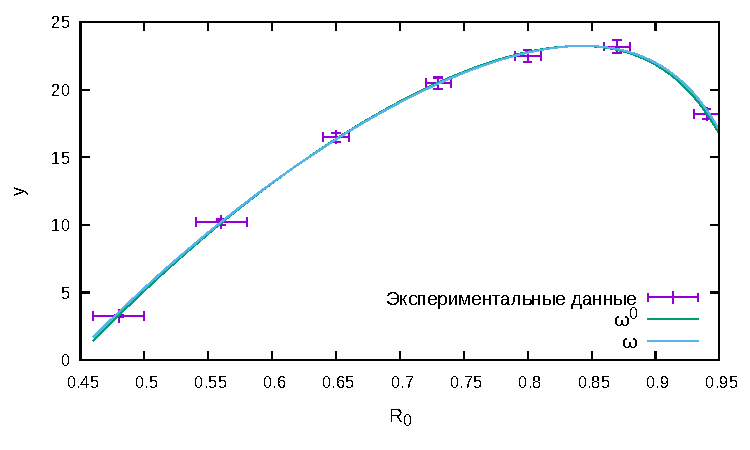
\includegraphics[width=\textwidth]{figs/levmar/results.pdf}
  \caption{Графики \eqref{eq:y_approx}, соответствующие параметрам,
	минимизирующим \eqref{eq:s} и \eqref{eq:s_classic}.}
  \label{fig:results}
\end{figure}

\subsection{Сходимость оптимальных параметров к классическим}
Численно исследована зависимость сходимости параметров $\bomega$ к параметрам $\bomega^0$,
получаемым минимизацией функционалов \eqref{eq:s} и \eqref{eq:s_classic} соответственно, от
погрешности $\mathbf{\sigma}_y$ измерения зависимой переменной $y$.

Следует ожидать, что при увеличении погрешности измерения величины $y$ при
фиксированной погрешности измерения $R_0$ оптимальный вектор $\bomega$
будет приближаться к $\bomega^0$, так как тем более незначителен
вклад ошибки измерения независимой переменной.

Рассматриваются два случая:
\begin{enumerate}
  \item Погрешность $i$-го измерения $y_i$ задается как $\sigma_{y_i} = 0.02ky_i$, т. е.
	погрешность зависит от значения самого $y_i$.
  \item Погрешность $i$-го измерения $y_i$ задается как $\sigma_{y_i} = 0.02ky_{\max}$,
	т. е. погрешность от значения конкретного $y_i$ не зависит. Заметим, что выбор
	конкретного значения $y$, определяющего погрешность, является в данном случае
	достаточно произвольным и соответствует умножению всех погрешностей на некоторую константу
	(что нивелируется соответствующим изменением выбора диапазона $k$).
\end{enumerate}

В первом случае ошибки измерения $y$ распределены неодинаково, следовательно, применение
стандартного метода наименьших квадратов не обосновано. В то же время во втором случае
ошибки принадлежат одному и тому же распределению, и, кроме того, независимы, поэтому
в данном случае МНК-оценка применима (с точностью до ошибки измерения независимой
переменной).

Для обоих случаев подробно рассматривалась область $k \in [1; 100]$, значение $k$
изменялось с шагом 0.01. Отметим, что уже при $k \approx 25$ характерная погрешность
измерения величины $y$ сопоставима с самой величиной $y$, а при $k > 50$ превышает ее.

Результаты приведены на рис. \ref{fig:conv_varY}.
На графиках отображены компоненты вектора $\bomega$, нормированные на
соответствующие значения $\bomega^0$, в зависимости от значения $k$.

\begin{figure}[h]
  \centering
  \begin{subfigure}[b]{0.5\textwidth}
    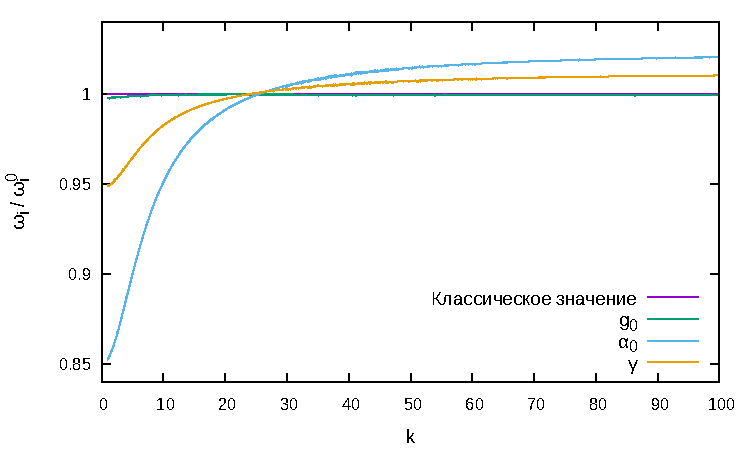
\includegraphics[width=\textwidth]{figs/levmar/convergence/convergence_1_100_0.01_yi.txt.pdf}
	\caption{$\sigma_{y_i} = 0.02ky_i$}
	\label{fig:conv_varY_100}
  \end{subfigure}%
  \begin{subfigure}[b]{0.5\textwidth}
    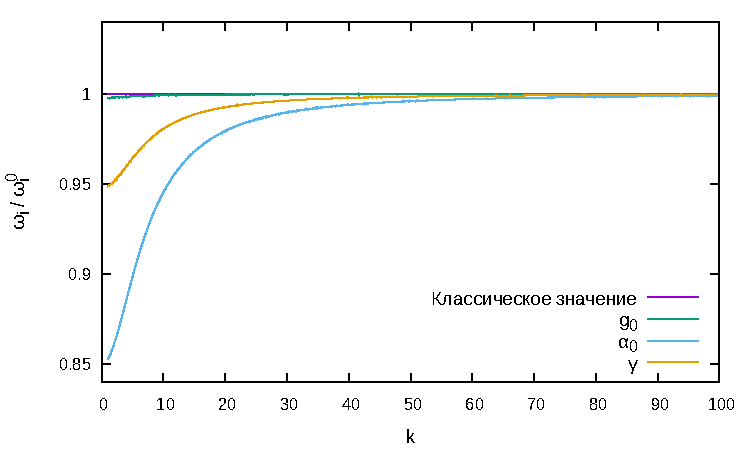
\includegraphics[width=\textwidth]{figs/levmar/convergence/convergence_1_100_0.01_ymax.txt.pdf}
	\caption{$\sigma_{y_i} = 0.02ky_{\max}$}
	\label{fig:conv_fixedY_100}
  \end{subfigure}
  \caption{Зависимость оптимальных параметров от $k \in [1; 100]$.}
  \label{fig:conv_varY}
\end{figure}

В случае фиксированной погрешности $\sigma_{y_i}$ значения $\bomega$
действительно стремятся к $\bomega^0$ для разумных значений $k$, а в случае
гетероскедастичных ошибок такой зависимости не наблюдается, хотя значения $\bomega$
и оказываются достаточно близки к $\bomega^0$. На наш взгляд, такое поведение
вектора оптимальных параметров является вполне ожидаемым и демонстрирует
несостоятельность классического функционала качества в случае неодинаково
распределенных ошибок.

\subsection{Сходимость параметров к истинным}
Численно исследована зависимость сходимости параметров $\bomega = \arg \min \breve{S}$
и $\bomega^0 = \arg \min S$ к некоторому <<истинному>> значению вектора параметров
$\hat{\bomega}$, от количества точек $\ell$ в обучающей выборке и от погрешности определения
независимой переменной.

Для этого вектор параметров $\bomega$, полученный минимизацией обучающей выборки из таблицы
\ref{tabl:measurements}, принимается за некоторый <<истинный>> вектор параметров $\hat{\bomega}$,
и на каждой $j$-й итерации генерируется обучающая выборка $D_j(\ell, k)$:
\[
  D_j(\ell, k) = \{ (x_i + \xi^x_i, y(x_i, \hat{\bomega}) + \xi^y_i) \} \mid \xi^x_i \sim \mathcal{N}(0, k \sigma_{x_i}), \xi^y_i \sim \mathcal{N}(0, \sigma_{y_i}), i \in \{ 1, \dots, \ell \},
\]
где $y(x, \bomega)$ задано соотношением \eqref{eq:y_approx}, а $\sigma_{x_i}$ и $\sigma_{y_i}$
определяются соотношением \eqref{eq:sigmas_definition}.

Иными словами, генерируется обучающая выборка согласно искомой модели с
известным и фиксированным вектором параметров, которая затем зашумляется нормально
распределенными случайными величинами. При этом стандартное отклонение
шума для зависимой величины совпадает с экспертно предложенной погрешностью
измерений для реального эксперимента, а стандартное отклонение независимой
величины отличается от экспертно предложенной погрешности для этой величины
в $k$ раз.

После генерации выборки $D_j(\ell, k)$ по ней находятся значения $\bomega_j = \arg \min \breve{S}(D_j)$
и $\bomega_j^0 = \arg \min S(D_j)$, что повторяется $N$ раз, и для $\forall i$ рассматриваются значения
\[
  \overline{\delta \omega_i} = \frac{\sum_{j = 1}^N (\omega_{ji} - \hat{\omega}_i)}{N},
\]
\[
  \overline{\delta \omega^0_i} = \frac{\sum_{j = 1}^N (\omega^0_{ji} - \hat{\omega}_i)}{N}.
\]

Обозначим, кроме того, $\overline{\delta \bomega} = \{ \overline{\delta \omega_1}, \overline{\delta \omega_2}, \overline{\delta \omega_3} \}$.

Таким образом, при варьировании $k$ и изучении поведения $\overline{\delta \bomega}$ и
$\overline{\delta \bomega^0}$ исследуется влияние погрешности определения
независимой переменной на разность между $\hat{\bomega}$ и оптимальными
параметрами $\bomega$ и $\bomega^0$ согласно \eqref{eq:s} и \eqref{eq:s_classic}
соответственно.

Так как при уменьшении $k$ монотонно уменьшается погрешность определения независимой
переменной, естественно ожидать, что различие между $\bomega$ и $\bomega^0$ будет
уменьшаться. Однако, наш вычислительный эксперимент демонстрирует, что это не так.

В нашем эксперименте $N = 1000$, $\ell \in \{ 10, \dots, 5000 \}$,
$k \in \{ 0.2, 0.25, \dots, 1 \}$.

Результаты приведены на рис. \ref{fig:comparison_0.2}-\ref{fig:comparison_gamma_k}.

\begin{figure}[h]
  \centering
  \begin{subfigure}[b]{0.35\textwidth}
    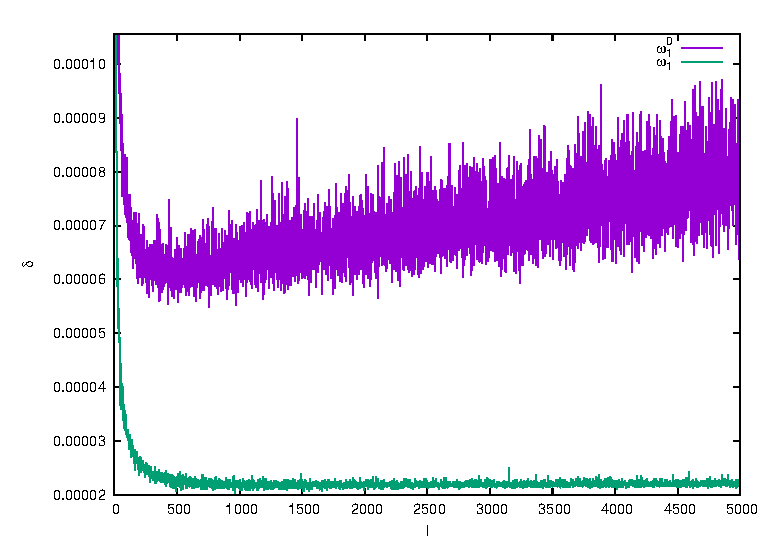
\includegraphics[width=\textwidth]{figs/levmar/comparison/comparison_5000_1000_xsigma0.20_float.txt_parameter1.eps}
	\caption{$g_0$}
  \end{subfigure}%
  \begin{subfigure}[b]{0.35\textwidth}
    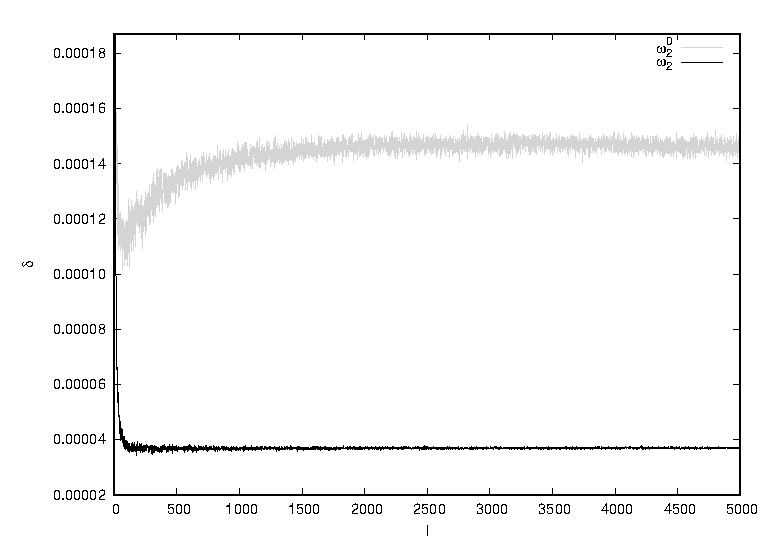
\includegraphics[width=\textwidth]{figs/levmar/comparison/comparison_5000_1000_xsigma0.20_float.txt_parameter2.eps}
	\caption{$\alpha_0$}
  \end{subfigure}%
  \begin{subfigure}[b]{0.35\textwidth}
    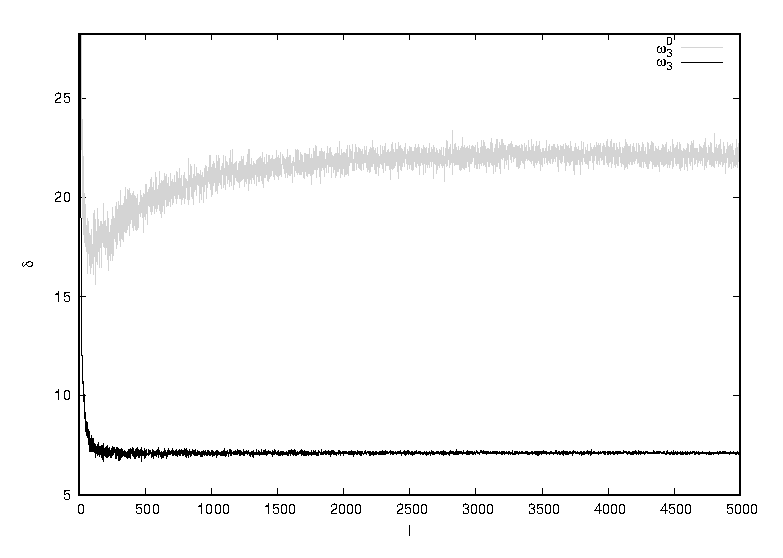
\includegraphics[width=\textwidth]{figs/levmar/comparison/comparison_5000_1000_xsigma0.20_float.txt_parameter3.eps}
	\caption{$\gamma$}
  \end{subfigure}
  \caption{Сходимость параметров к истинным при $k = 0.2$.}
  \label{fig:comparison_0.2}
\end{figure}

\begin{figure}[h]
  \centering
  \begin{subfigure}[b]{0.35\textwidth}
    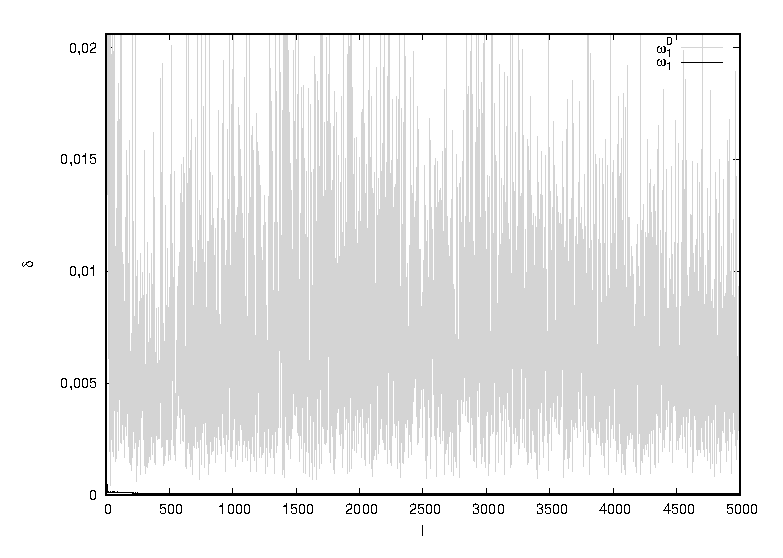
\includegraphics[width=\textwidth]{figs/levmar/comparison/comparison_5000_1000_xsigma0.65_float.txt_parameter1.eps}
	\caption{$g_0$}
	\label{fig:comparison_0.65_g0}
  \end{subfigure}%
  \begin{subfigure}[b]{0.35\textwidth}
    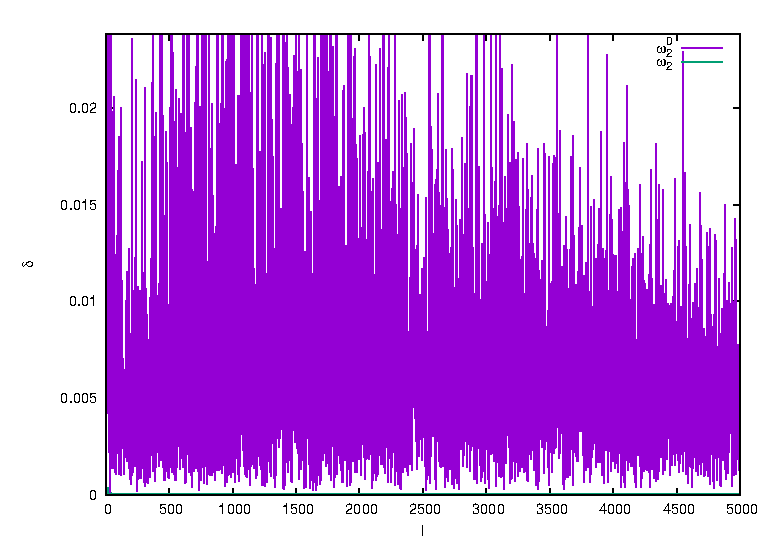
\includegraphics[width=\textwidth]{figs/levmar/comparison/comparison_5000_1000_xsigma0.65_float.txt_parameter2.eps}
	\caption{$\alpha_0$}
	\label{fig:comparison_0.65_alpha0}
  \end{subfigure}%
  \begin{subfigure}[b]{0.35\textwidth}
    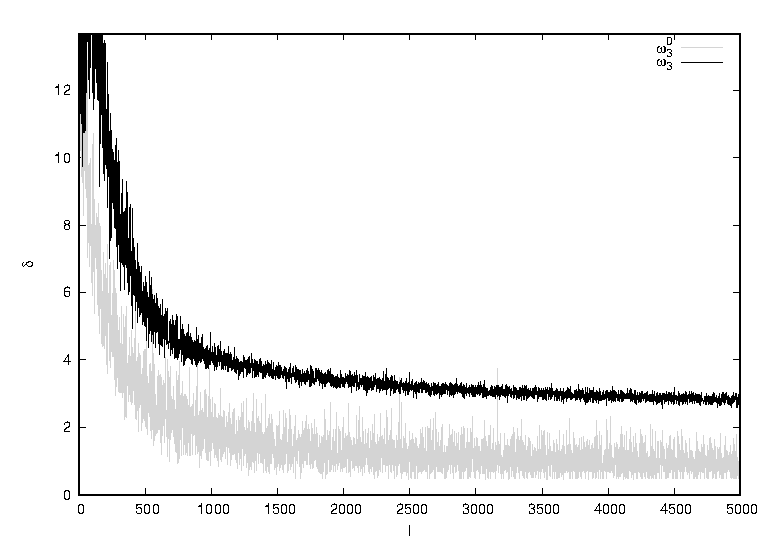
\includegraphics[width=\textwidth]{figs/levmar/comparison/comparison_5000_1000_xsigma0.65_float.txt_parameter3.eps}
	\caption{$\gamma$}
  \end{subfigure}
  \caption{Сходимость параметров к истинным при $k = 0.65$.}
  \label{fig:comparison_0.65}
\end{figure}

\begin{figure}[h]
  \centering
  \begin{subfigure}[b]{0.35\textwidth}
    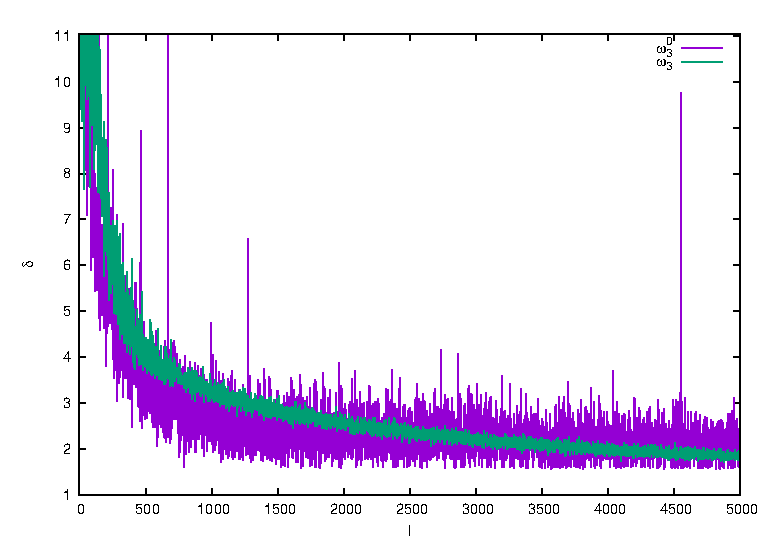
\includegraphics[width=\textwidth]{figs/levmar/comparison/comparison_5000_1000_xsigma0.80_float.txt_parameter3.eps}
	\caption{$k = 0.8$}
  \end{subfigure}%
  \begin{subfigure}[b]{0.35\textwidth}
    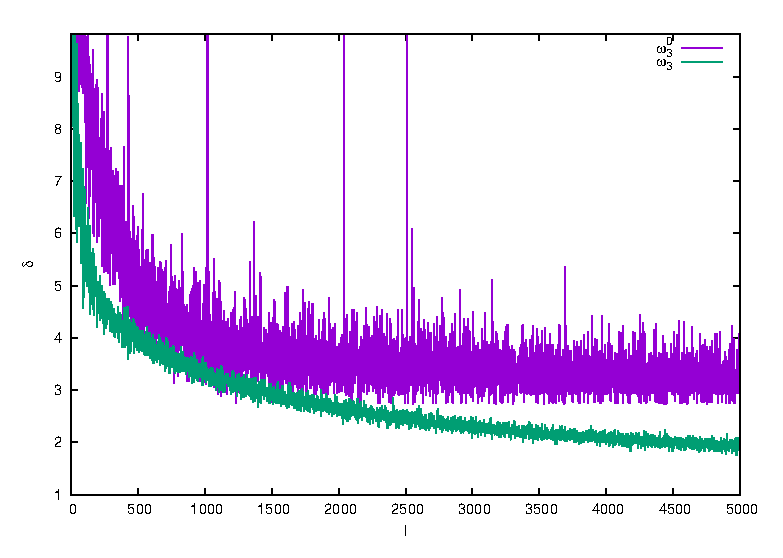
\includegraphics[width=\textwidth]{figs/levmar/comparison/comparison_5000_1000_xsigma0.90_float.txt_parameter3.eps}
	\caption{$k = 0.9$}
  \end{subfigure}%
  \begin{subfigure}[b]{0.35\textwidth}
    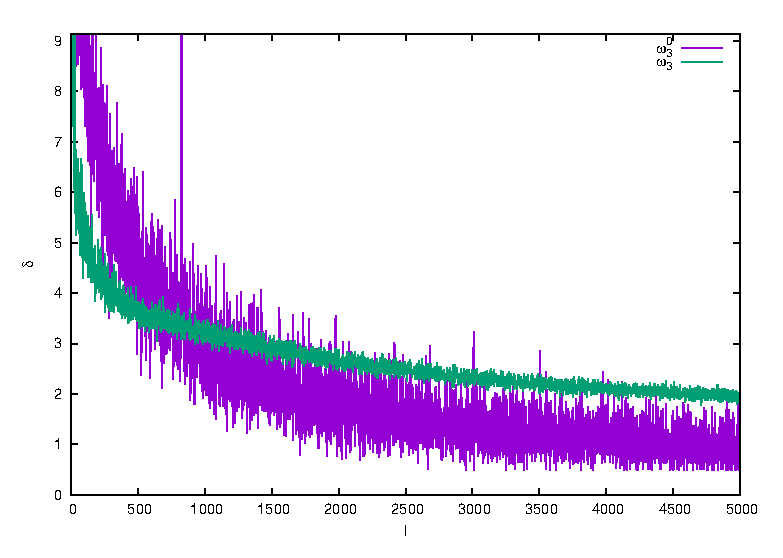
\includegraphics[width=\textwidth]{figs/levmar/comparison/comparison_5000_1000_xsigma1.00_float.txt_parameter3.eps}
	\caption{$k = 1.0$}
  \end{subfigure}
  \caption{Сходимость параметра $\gamma$ при некоторых $k$.}
  \label{fig:comparison_gamma_k}
\end{figure}

Результаты на рис. \ref{fig:comparison_0.2} характерны для всех
значений $k \in [0.2, 0.6]$. Однако, при $k \geq 0.65$ поведение оптимальных
параметров резко меняется. Так, на рис. \ref{fig:comparison_0.65} приведены
графики сходимости для $k = 0.65$. Видно, что поведение параметров,
оптимизированных согласно классическому функционалу качества $S$, является
существенно более хаотическим, что может говорить о меньшей устойчивости
\cite{Rudoy16StabilityAnalysis} модели, оптимизированной согласно $S$.

Более того, для оценок параметров $g_0$ и $\alpha_0$ соответствующее
приближение на несколько порядков хуже, чем полученное минимизацией $\breve{S}$,
вплоть до того, что кривые, соответствующие минимизирующим $\breve{S}$ параметрам,
практически не видно на графиках (рис. \ref{fig:comparison_0.65_g0} и
\ref{fig:comparison_0.65_alpha0}), поскольку в выбранном масштабе они
практически совпадают с осью абсцисс. С другой стороны, важно отметить, что оценка
параметра $\gamma$, полученная минимизацией $S$, является несколько лучшей для
$k = 0.65$ (для $k = 0.7$ график выглядит аналогично), но минимизация $\breve{S}$
дает все лучшие и лучшие приближения с ростом $k$ (рис.
\ref{fig:comparison_gamma_k}).

Отметим следующее:
\begin{itemize}
  \item Практически во всех случаях (кроме оценки $\gamma$ для $k = 0.8$)
	предложенный в настоящей работе функционал \eqref{eq:s}
	дает лучшее приближение, в том числе, при разумно малом объеме обучающей выборки. Кроме того, в
	подавляющем большинстве случаев предпочтительность предложенного функционала
	сохраняется и для большего числа экспериментальных точек.
  \item Для малых $k \leq 0.6$ ошибка оценки параметров при помощи классического
	функционала \eqref{eq:s_classic} имеет ярко выраженный минимум в окрестности 60-100
	для $\alpha_0$ и $\gamma$ и 400 для $g_0$ экспериментальных точек
	(рис. \ref{fig:comparison_0.2}).
	Дальнейшее увеличение обучающей выборки ведет к ухудшению приближения, получаемого
	минимизацией \eqref{eq:s_classic}.
  \item Для некоторых $k$ ошибка приближения, получаемого минимизацией предложенного
	функционала \eqref{eq:s}, имеет явную горизонтальную асимптоту (рис. \ref{fig:comparison_0.2},
	\ref{fig:comparison_0.65_g0} и \ref{fig:comparison_0.65_alpha0}).
\end{itemize}

Причины подобного поведения оптимальных параметров являются предметом
дальнейших исследований.

\section{Заключение}

Предложен модифицированный функционал среднеквадратичной ошибки для задач
регрессии, применимый в случае наличия ошибок измерения независимых
переменных и различных распределений, к которым принадлежат ошибки, в разных
точках обучающей выборки. Предложена вероятностная интерпретация этого
функционала для случая нормального распределения ошибок измерения.

Показана сходимость предложенного функционала к классическому функционалу
среднеквадратичной ошибки для случая гомоскедастичности погрешностей
зависимой переменной и пренебрежимо малой погрешности измерения независимых
переменных.

Исследовано поведение оптимального вектора параметров для предлагаемого
функционала в зависимости от параметров распределений ошибок независимых
переменных, в том числе, в сравнении с вектором параметров, минимизирующим
классический функционал качества.

Представляется разумным использовать предложенный в настоящей работе функционал
качества при оптимизации параметров регрессионных моделей и анализе их
устойчивости к погрешностям как зависимых, так и независимых
переменных\cite{Rudoy15MonteCarlo,Rudoy16StabilityAnalysis}.

\FloatBarrier

\bibliographystyle{babunsrt-lf}
\bibliography{bibliography}

\begin{center}
  \rule{\textwidth}{1pt}
  \rule{\textwidth}{1pt}
\end{center}

\begin{center}
  \uppercase{On modification of the MSE loss function for solving non-linear heteroscedastic errors-in-variables problems}

  \bigskip
  G.~Rudoy$^1$
\end{center}

$^1$Moscow Institute of Physics and Technology, 9 Institutskiy Per.,
Dolgoprudny, Moscow Region 141700, Russian Federation

\renewcommand{\abstractname}{Abstract}

\begin{abstract}
  The paper considers the problem of finding the optimal parameters of a
  non-linear regression model accounting for errors in both dependent and
  independent variables. The errors of different measurements are assumed to
  belong to different probability distributions with different variances.
  A modified mean squared error-based loss function is derived and analyzed
  for this case.

  In the computational experiment the measurements of the laser's radiation
  power as a non-linear function of the resonator's transparency are used to
  compare the parameters vectors minimizing the presented
  loss function and the classical mean squared error.
  The convergence of the parameters minimizing the presented loss function
  to the optimal parameters for the classical loss function is studied.
  In addition, some values of the parameters are considered to be <<true>>
  ones and are used to generate synthetic data using the physical model and
  Gaussian noise, which is then used to study the convergence of the parameters
  minimizing the presented and the classical loss function, respectively, as
  the function of the noise parameters.

  \textbf{Keywords}: \emph{errors-in-variables models, heteroscedastic errors,
  symbolic regression, non-linear regression}.
\end{abstract}

\renewcommand{\refname}{References}
\begin{thebibliography}{1}
  \providebibliographyfont{name}{}%
  \providebibliographyfont{lastname}{}%
  \providebibliographyfont{title}{\emph}%
  \providebibliographyfont{jtitle}{\btxtitlefont}%
  \providebibliographyfont{etal}{\emph}%
  \providebibliographyfont{journal}{}%
  \providebibliographyfont{volume}{}%
  \providebibliographyfont{ISBN}{\MakeUppercase}%
  \providebibliographyfont{ISSN}{\MakeUppercase}%
  \providebibliographyfont{url}{\url}%
  \providebibliographyfont{numeral}{}%
  \expandafter\btxselectlanguage\expandafter {\btxfallbacklanguage}

\btxselectlanguage {english}
\bibitem {Rudoy15MonteCarlo-en}
\btxnamefont {\btxlastnamefont {Rudoy}, G.\btxfnamespacelong
  I.}\btxauthorcolon\ \btxjtitlefont {\btxifchangecase {Applying
	Monte Carlo methods to analysis of nonlinear regression
	models}{Applying Monte Carlo methods to analysis of nonlinear
	regression models}}.
\newblock \btxjournalfont {Numerical Analysis and
	Applications}, 4:344--350, 2015.

\btxselectlanguage {english}
\bibitem {jukic2013nonlinear-en}
\btxnamefont {\btxlastnamefont {Juki\'{c}}, Dragan}\btxauthorcolon\
  \btxjtitlefont {\btxifchangecase {On nonlinear weighted least squares
  estimation of bass diffusion model}{On nonlinear weighted least squares
  estimation of Bass diffusion model}}.
\newblock \btxjournalfont {Applied mathematics and computation},
  219(14):7891--7900, 2013.

\btxselectlanguage {english}
\bibitem {jukic2010nonlinear-en}
\btxnamefont {\btxlastnamefont {Juki{\'c}}, Dragan} \btxandlong {}\
  \btxnamefont {\btxlastnamefont {Markovi{\'c}}, Darija}\btxauthorcolon\
  \btxjtitlefont {\btxifchangecase {On nonlinear weighted errors-in-variables
  parameter estimation problem in the three-parameter weibull model}{On
  nonlinear weighted errors-in-variables parameter estimation problem in the
  three-parameter Weibull model}}.
\newblock \btxjournalfont {Applied mathematics and computation},
  215(10):3599--3609, 2010.

\btxselectlanguage {english}
\bibitem {kiryati2000heteroscedastic-en}
\btxnamefont {\btxlastnamefont {Kiryati}, Nahum} \btxandlong {}\ \btxnamefont
  {\btxlastnamefont {Bruckstein}, Alfred\btxfnamespacelong M}\btxauthorcolon\
  \btxjtitlefont {\btxifchangecase {Heteroscedastic hough transform (htht): An
  efficient method for robust line fitting in the {\lq}errors in the
  variables{\rq} problem}{Heteroscedastic Hough transform (HtHT): An efficient
  method for robust line fitting in the {\lq}errors in the variables{\rq}
  problem}}.
\newblock \btxjournalfont {Computer Vision and Image Understanding},
  78(1):69--83, 2000.

\btxselectlanguage {english}
\bibitem {Marquardt1963Algorithm-en}
\btxnamefont {\btxlastnamefont {Marquardt}, D.\btxfnamespacelong
  W.}\btxauthorcolon\ \btxjtitlefont {\btxifchangecase {An algorithm for
  least-squares estimation of non-linear parameters}{An Algorithm for
  Least-squares Estimation of Non-linear Parameters}}.
\newblock \btxjournalfont {Journal of the Society of Industrial and Applied
  Mathematics}, 11(2):431--441, 1963.

\btxselectlanguage {english}
\bibitem {dlib09-en}
\btxnamefont {\btxlastnamefont {King}, Davis\btxfnamespacelong
  E.}\btxauthorcolon\ \btxjtitlefont {\btxifchangecase {Dlib-ml: A machine
  learning toolkit}{Dlib-ml: A Machine Learning Toolkit}}.
\newblock \btxjournalfont {Journal of Machine Learning Research},
  10:1755--1758, 2009.

\btxselectlanguage {english}
\bibitem {alexandrov1991kinetics-en}
\btxnamefont {\btxlastnamefont {Aleksandrov}, A.\btxfnamespacelong
  Yu.}, \btxnamefont {\btxlastnamefont {Dolgikh}, V.\btxfnamespacelong
  A.}\btxandcomma {} \btxetalfont {\btxetalshort {.}}\btxauthorcolon\
  \btxjtitlefont {\btxifchangecase {Kinetika vozbuzhdaemogo elektronnym
  puchkom lazera vysokogo davleniya na" zheltoy" linii neona}{Kinetika
  vozbuzhdaemogo elektronnym puchkom lazera vysokogo davleniya na" zheltoy" linii neona}}.
\newblock \btxjournalfont {Kvantovaya elektronika},
  18(9):1029--1033, 1991.

\btxselectlanguage {english}
\bibitem {champagne1982transient-en}
\btxnamefont {\btxlastnamefont {Champagne}, LF}\btxauthorcolon\ \btxtitlefont
  {\btxifchangecase {Transient optical absorption in the ultraviolet}{Transient
  Optical Absorption in the Ultraviolet}}.
\newblock \Btxinlong {}\ \btxnamefont {\btxlastnamefont {McDaniel},
  E.\btxfnamespacelong W.} \btxandlong {}\ \btxnamefont {\btxlastnamefont
  {Nighan}, William\btxfnamespacelong L.}\ (\btxeditorslong {}): \btxtitlefont
  {Applied Atomic Collision Physics, Volume 3: Gas Lasers}, \btxvolumelong
  {}~\btxvolumefont {3}, \btxpageslong {}\ 349--386, 1982.

\btxselectlanguage {english}
\bibitem {Rudoy16StabilityAnalysis-en}
\btxnamefont {\btxlastnamefont {Rudoy}, G.\btxfnamespacelong
  I.}\btxauthorcolon\ \btxjtitlefont {\btxifchangecase {Analysis of the
  stability of nonlinear regression models to errors in measured data}{Analysis
  of the stability of nonlinear regression models to errors in measured data}}.
\newblock \btxjournalfont {Pattern Recognition and Image Analysis}, 26(3):608--616,
  2016.

\end{thebibliography}

\section*{Contributors}

\textbf{Rudoy Georg I.} (b. 1991)~-- PhD student,
Moscow Institute of Physics and Technology, 9 Institutskiy Per., Dolgoprudny,
Moscow Region 141700, Russian Federation;
0xd34df00d@gmail.com

\end{document}
